\documentclass{ximera}

%\usepackage{todonotes}

\newcommand{\todo}{}

\usepackage{esint} % for \oiint
\graphicspath{
  {./}
  {ximeraTutorial/}
}

\newcommand{\mooculus}{\textsf{\textbf{MOOC}\textnormal{\textsf{ULUS}}}}

\usepackage{tkz-euclide}
\tikzset{>=stealth} %% cool arrow head
\tikzset{shorten <>/.style={ shorten >=#1, shorten <=#1 } } %% allows shorter vectors

\usetikzlibrary{backgrounds} %% for boxes around graphs
\usetikzlibrary{shapes,positioning}  %% Clouds and stars
\usetikzlibrary{matrix} %% for matrix
\usepgfplotslibrary{polar} %% for polar plots
\usetkzobj{all}
\usepackage[makeroom]{cancel} %% for strike outs
%\usepackage{mathtools} %% for pretty underbrace % Breaks Ximera
\usepackage{multicol}
\usepackage{pgffor} %% required for integral for loops


%% http://tex.stackexchange.com/questions/66490/drawing-a-tikz-arc-specifying-the-center
%% Draws beach ball 
\tikzset{pics/carc/.style args={#1:#2:#3}{code={\draw[pic actions] (#1:#3) arc(#1:#2:#3);}}}



\usepackage{array}
\setlength{\extrarowheight}{+.1cm}   
\newdimen\digitwidth
\settowidth\digitwidth{9}
\def\divrule#1#2{
\noalign{\moveright#1\digitwidth
\vbox{\hrule width#2\digitwidth}}}





\newcommand{\RR}{\mathbb R}
\newcommand{\R}{\mathbb R}
\newcommand{\N}{\mathbb N}
\newcommand{\Z}{\mathbb Z}

\newcommand{\sagemath}{\textsf{SageMath}}


%\renewcommand{\d}{\,d\!}
\renewcommand{\d}{\mathop{}\!d}
\newcommand{\dd}[2][]{\frac{\d #1}{\d #2}}
\newcommand{\pp}[2][]{\frac{\partial #1}{\partial #2}}
\renewcommand{\l}{\ell}
\newcommand{\ddx}{\frac{d}{\d x}}

\newcommand{\zeroOverZero}{\ensuremath{\boldsymbol{\tfrac{0}{0}}}}
\newcommand{\inftyOverInfty}{\ensuremath{\boldsymbol{\tfrac{\infty}{\infty}}}}
\newcommand{\zeroOverInfty}{\ensuremath{\boldsymbol{\tfrac{0}{\infty}}}}
\newcommand{\zeroTimesInfty}{\ensuremath{\small\boldsymbol{0\cdot \infty}}}
\newcommand{\inftyMinusInfty}{\ensuremath{\small\boldsymbol{\infty - \infty}}}
\newcommand{\oneToInfty}{\ensuremath{\boldsymbol{1^\infty}}}
\newcommand{\zeroToZero}{\ensuremath{\boldsymbol{0^0}}}
\newcommand{\inftyToZero}{\ensuremath{\boldsymbol{\infty^0}}}



\newcommand{\numOverZero}{\ensuremath{\boldsymbol{\tfrac{\#}{0}}}}
\newcommand{\dfn}{\textbf}
%\newcommand{\unit}{\,\mathrm}
\newcommand{\unit}{\mathop{}\!\mathrm}
\newcommand{\eval}[1]{\bigg[ #1 \bigg]}
\newcommand{\seq}[1]{\left( #1 \right)}
\renewcommand{\epsilon}{\varepsilon}
\renewcommand{\phi}{\varphi}


\renewcommand{\iff}{\Leftrightarrow}

\DeclareMathOperator{\arccot}{arccot}
\DeclareMathOperator{\arcsec}{arcsec}
\DeclareMathOperator{\arccsc}{arccsc}
\DeclareMathOperator{\si}{Si}
\DeclareMathOperator{\proj}{\vec{proj}}
\DeclareMathOperator{\scal}{scal}
\DeclareMathOperator{\sign}{sign}


%% \newcommand{\tightoverset}[2]{% for arrow vec
%%   \mathop{#2}\limits^{\vbox to -.5ex{\kern-0.75ex\hbox{$#1$}\vss}}}
\newcommand{\arrowvec}{\overrightarrow}
%\renewcommand{\vec}[1]{\arrowvec{\mathbf{#1}}}
\renewcommand{\vec}{\mathbf}
\newcommand{\veci}{{\boldsymbol{\hat{\imath}}}}
\newcommand{\vecj}{{\boldsymbol{\hat{\jmath}}}}
\newcommand{\veck}{{\boldsymbol{\hat{k}}}}
\newcommand{\vecl}{\boldsymbol{\l}}
\newcommand{\uvec}[1]{\mathbf{\hat{#1}}}
\newcommand{\utan}{\mathbf{\hat{t}}}
\newcommand{\unormal}{\mathbf{\hat{n}}}
\newcommand{\ubinormal}{\mathbf{\hat{b}}}

\newcommand{\dotp}{\bullet}
\newcommand{\cross}{\boldsymbol\times}
\newcommand{\grad}{\boldsymbol\nabla}
\newcommand{\divergence}{\grad\dotp}
\newcommand{\curl}{\grad\cross}
%\DeclareMathOperator{\divergence}{divergence}
%\DeclareMathOperator{\curl}[1]{\grad\cross #1}
\newcommand{\lto}{\mathop{\longrightarrow\,}\limits}

\renewcommand{\bar}{\overline}

\colorlet{textColor}{black} 
\colorlet{background}{white}
\colorlet{penColor}{blue!50!black} % Color of a curve in a plot
\colorlet{penColor2}{red!50!black}% Color of a curve in a plot
\colorlet{penColor3}{red!50!blue} % Color of a curve in a plot
\colorlet{penColor4}{green!50!black} % Color of a curve in a plot
\colorlet{penColor5}{orange!80!black} % Color of a curve in a plot
\colorlet{penColor6}{yellow!70!black} % Color of a curve in a plot
\colorlet{fill1}{penColor!20} % Color of fill in a plot
\colorlet{fill2}{penColor2!20} % Color of fill in a plot
\colorlet{fillp}{fill1} % Color of positive area
\colorlet{filln}{penColor2!20} % Color of negative area
\colorlet{fill3}{penColor3!20} % Fill
\colorlet{fill4}{penColor4!20} % Fill
\colorlet{fill5}{penColor5!20} % Fill
\colorlet{gridColor}{gray!50} % Color of grid in a plot

\newcommand{\surfaceColor}{violet}
\newcommand{\surfaceColorTwo}{redyellow}
\newcommand{\sliceColor}{greenyellow}




\pgfmathdeclarefunction{gauss}{2}{% gives gaussian
  \pgfmathparse{1/(#2*sqrt(2*pi))*exp(-((x-#1)^2)/(2*#2^2))}%
}


%%%%%%%%%%%%%
%% Vectors
%%%%%%%%%%%%%

%% Simple horiz vectors
\renewcommand{\vector}[1]{\left\langle #1\right\rangle}


%% %% Complex Horiz Vectors with angle brackets
%% \makeatletter
%% \renewcommand{\vector}[2][ , ]{\left\langle%
%%   \def\nextitem{\def\nextitem{#1}}%
%%   \@for \el:=#2\do{\nextitem\el}\right\rangle%
%% }
%% \makeatother

%% %% Vertical Vectors
%% \def\vector#1{\begin{bmatrix}\vecListA#1,,\end{bmatrix}}
%% \def\vecListA#1,{\if,#1,\else #1\cr \expandafter \vecListA \fi}

%%%%%%%%%%%%%
%% End of vectors
%%%%%%%%%%%%%

%\newcommand{\fullwidth}{}
%\newcommand{\normalwidth}{}



%% makes a snazzy t-chart for evaluating functions
%\newenvironment{tchart}{\rowcolors{2}{}{background!90!textColor}\array}{\endarray}

%%This is to help with formatting on future title pages.
\newenvironment{sectionOutcomes}{}{} 



%% Flowchart stuff
%\tikzstyle{startstop} = [rectangle, rounded corners, minimum width=3cm, minimum height=1cm,text centered, draw=black]
%\tikzstyle{question} = [rectangle, minimum width=3cm, minimum height=1cm, text centered, draw=black]
%\tikzstyle{decision} = [trapezium, trapezium left angle=70, trapezium right angle=110, minimum width=3cm, minimum height=1cm, text centered, draw=black]
%\tikzstyle{question} = [rectangle, rounded corners, minimum width=3cm, minimum height=1cm,text centered, draw=black]
%\tikzstyle{process} = [rectangle, minimum width=3cm, minimum height=1cm, text centered, draw=black]
%\tikzstyle{decision} = [trapezium, trapezium left angle=70, trapezium right angle=110, minimum width=3cm, minimum height=1cm, text centered, draw=black]


\title{Which Way?}

\begin{document}

\begin{abstract}
%Stuff can go here later if we want!
\end{abstract}

\maketitle





Given two sets and connections between their members, we always have a relation. But, we don't always have a function. The extra rule can be a kink at times. 


\begin{example}
Here is a diagram of two sets and line segments illustrating the connections.

\begin{center}
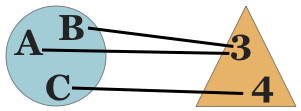
\includegraphics{pics/func.png}
\end{center}
\quad \\


We naturally read left to right, so it is common to see 
\includegraphics{pics/circle.png} as the domain and 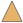
\includegraphics{pics/triangle.png} as the range.  The pairs would be 
\[
\{ (A, 3), (B, 3), (C, 4) \}
\]


But, we could just as easily see 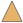
\includegraphics{pics/triangle.png} as the domain and 
\includegraphics{pics/circle.png} as the range.  Then the pairs would be
\[
\{ (3, A), (3, B), (4, C) \}
\]


Either one is ok. Both are relations. \\
However, they are not both functions. \\
\quad \\

The pairs $\{ (A, 3), (B, 3), (C, 4) \}$ follow the rule for a function. \\
We would think that 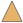
\includegraphics{pics/triangle.png} is a \textbf{function} of 
\includegraphics{pics/circle.png}. The function value in 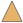
\includegraphics{pics/triangle.png} depends on the value in 
\includegraphics{pics/circle.png}. \\


The pairs $\{ (3, A), (3, B), (4, C) \}$ do not follow the rule for a function.  \\
3 is in the domain and it is in two different pairs. We would think that 
\includegraphics{pics/circle.png} is not a function of 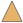
\includegraphics{pics/triangle.png}.

\end{example}

\quad \\


For a function, not only is the connection between the sets important, but it is just as important to designate which set is the domain and which is the range. \\
Which way does the function go?

\begin{example}
\quad \\
\begin{itemize}
\item Ice Cream Flavors is a function of kindergarteners. \\
Kindergarteners is the domain and each kindergartener is paired with exactly one ice cream flavor. 

\item Kindergarteners is not a function of ice cream flavors. \\
Chocolate would be in the domain and paired with six kindergarteners.

\item Grocery Store Prices is a function of products.\\
Each item in the store is paired with exactly one price. 

\item Grocery Store Products is not a function of prices.\\
\$1.24 would be a price in the domain that is paired with multiple products.

\item State Flags is a function of states.\\
Each state in the domain is paired with exactly one flag.

\item State Flags is also a function of State flags.\\
Each state flag in the domain is paired with exactly one state.
\end{itemize}

\end{example}
\quad \\



To create a function, you have to actually identify the domain and range explicitly and then the pairs.


\begin{definition}
A package containing three sets is either a function or it is not.  It is a simple yes/no question.  If the answer is "yes", then we say the function is \textbf{well-defined}.  If the answer is "no", then we say the function is \textbf{ not well-defined}.
\end{definition}


\begin{remark} COMMUNICATION \\
We say that the codomain or range is a function of the domain.
We naturally think to pick a domain number first and then see which codomain/range item results.  So, we say that the codomain/range depends on the domain.
\end{remark}


There are many different ways to break the function rule.

\begin{example}
These both break the function rule. \\
\quad \\
\begin{itemize}
\item Domain : $\{ A, B, C \}$
\item Codomain : $\{ 3, 4, 5 \}$
\item Pairs : $\{ (A, 4), (C, 5) \}$
\end{itemize}
$B$ is in the domain and not in a pair.

\begin{itemize}
\item Domain : $\{ A, B, C \}$
\item Codomain : $\{ 3, 4, 5 \}$
\item Pairs : $\{ (A, 4), (C, 5) , (B, 4), (A, 5) \}$
\end{itemize}
$A$ is in the domain and is in more than one pair.
\end{example}
\quad \\


\begin{question}
\begin{itemize}
\item Domain : $\{ A, B, C \}$
\item Codomain : $\{ 3, 4, 5 \}$
\item Pairs : $\{ (A, 3), (B, 3), (C, 3) \}$
\end{itemize}

\begin{multipleChoice}
\choice[correct]{Well-Defined}
\choice{Not Well-Defined}
\end{multipleChoice}
\begin{feedback}
Every domain item is in exactly one pair. 
\end{feedback}
\end{question}



\begin{question}
\begin{itemize}
\item Domain : $\{ A, B, C \}$
\item Codomain : $\{ 3, 4, 5 \}$
\item Pairs : $\{ (A, 7), (B, 3), (C, 3) \}$
\end{itemize}

\begin{multipleChoice}
\choice{Well-Defined}
\choice[correct]{Not Well-Defined}
\end{multipleChoice}
\begin{feedback}
$7$ is not in the codomain and not available to be paired with $A$.. 
\end{feedback}
\end{question}




\begin{question}
\begin{itemize}
\item Domain : $\{ A, B, C \}$
\item Codomain : $\{ 3, 4, 5 \}$
\item Pairs : $\{ (A, 7), (B, 3), (C, 3), (D, 5) \}$
\end{itemize}

\begin{multipleChoice}
\choice{Well-Defined}
\choice[correct]{Not Well-Defined}
\end{multipleChoice}
\begin{feedback}
$D$ is not in the domain and not available to be paired with $A$..
\end{feedback}
\end{question}


\begin{question}
\begin{itemize}
\item Domain : $?$
\item Codomain : $\{ 3, 4, 5 \}$
\item Pairs : $\{ (A, 3), (B, 4), (C, 5) \}$
\end{itemize}

\begin{multipleChoice}
\choice{Well-Defined}
\choice{Not Well-Defined}
\choice[correct]{not enough information}
\end{multipleChoice}
\begin{feedback}
The pairs suggest a well-defined function, but we need to know the domain to make sure.
\end{feedback}
\end{question}



\begin{example}
These both satisfy the function rule. \\
\quad \\
\begin{itemize}
\item Domain : $\{ A, B, C \}$
\item Codomain : $\{ 3, 4, 5 \}$
\item Pairs : $\{ (A, 4), (B, 5), (C, 4) \}$
\end{itemize}
$3$ is in the codomain and not in a pair, but the rule was not concerned with codomain items, just domain items.

\begin{itemize}
\item Domain : $\{ A, B, C \}$
\item Codomain : $\{ 3, 4, 5 \}$
\item Pairs : $\{ (A, 4), (C, 5) , (B, 4), (A, 4) \}$
\end{itemize}
$A $is in the domain and appears in more than one pair, except it doesn?t. The same pair is just written twice.  There is no rule about how many times you can write something.  We are only concerned with $A$ being paired with more than one codomain item.
\end{example}
\quad \\








\end{document}
